\section{Different $\mu$, $\sigma$, $\lambda$ Verification}
The whole Lévy process $X_t$ can be treated as normal Brownian motion($X_{t}=\mu t+\sigma B_{t}$) plus a jump ($\sum_{i=1}^{N_{t}} Y_{i}$). In general, $\mu$ contributes to the linear drift and $\sigma$ is relevant to the motion variance. The jump magnitude is controlled by $Y_i$.

The jump arrival time interval $T$ is an exponential distribution with $\lambda$. The total time $S$ is accumulation of $T$ which is an Erlang distribution with parameters of jump numbers and $\lambda$. For this reason, the last jump arrival time is stochastic in each simulation.

Because $\mu$ and $\sigma$ influences normal Brownian motion only so the jump element can be excluded when investigating independent different values of $\mu$ and $\sigma$. According to the characteristics of Brownian motion, in any time $S$, the mean value of the change of $X_t$ is 
$$ E(\mu t+\sigma B_{S})=\mu S+\sigma E(B_S)$$
Because $B_S$ is standard Brownian motion subjects to normal distribution with mean is $0$, $E(B_S)=0$. So the final mean value is $\mu S$.

Regarding to variance, it can be calculated by
$$V[\mu t+\sigma B_{t}]=V[\mu S]+V[\sigma B_{S}]+2Cov[B_{S}, S]$$
where
$$V[\mu S]=\mu^2 V[S] $$
$$V[\sigma B_S]=\sigma^2(E[V(B_S|S]] + V[E[B_S|S]])= \sigma^2 E[S]$$
$$Cov[B_{S}, S]=E[S*B_S] – E[S]E[B_S] = E[S*B_S]=0$$

Remind that S follows Erlang distribution with $\lambda$ $$V[S]=\frac{Total Jump Numbers}{\lambda^2}$$
$$E[S]=\frac{Total Jump Numbers}{\lambda}$$

So the final variance
$$V[\mu t+\sigma B_{t}]=\mu^2 {\frac{Total Jump Numbers}{\lambda^2}}+ \sigma^2 {\frac{Total Jump Numbers}{\lambda}}$$

Assume that the jump $Y_i$ is an exponential distribution of $\lambda_Y=1$ in simulation. In this case it is quite obvious that the motion will reach higher if $\lambda_Y$ increases. But if the $\mu$ changes in opposite direction of $\lambda_Y$, the motion will be pull back. The detailed analysis of this is described \ref{4.4} .

\subsection{Different $\mu$}
To verify how $\mu$ influences the motion, we like to keep the $\sigma$ and $\lambda$ as constant, in simulation both $\sigma$ and $\lambda$ are set to 1.

In the case of $\mu>0$ the path slope goes up as $\mu$ increases and vice verse. When the $\mu$ is extreme small($10^{-5}$) the path is similar to the Brownian motion without linear drift but the motion path is dominated by linear drift if $\mu$ is very large ($10^{5}$). The simulation result is shown on Figure \ref{fig:diffmu}

Consider the case $\mu=10^{5}$, the simulation generates 100 $A_{1000}$ at time $S_{1000}$ (since each run the last arrival time is scholastic so $S_{1000}$ is calculated as a mean of 100 last arrival time). The result of mean of 100 $A_{1000}$ is $1.0001\times 10^8$ and the theoretical calculation $\mu S_{1000}$ is $9.9926\times 10^7$, they are nearly the same.

When the $\mu=10^{-5}$, it is close to 0, the motion variance becomes very large because there is almost no linear drift. The theoretical mean value of $A_{1000}$ in 100 runs is $0.01$ but the actual mean of $A_{1000}$ is approximate -1.12, this is since the sample is only 100 and if it is increased to 100000, the mean of $A_{1000}$ is $0.018$ is improved to very close to the theoretical value.

Apparently if $\mu<0$ the motion will move to the negative $y$ axles and the slope reduces as $\mu$ decreases.  

\begin{figure}[H]
    \centering
    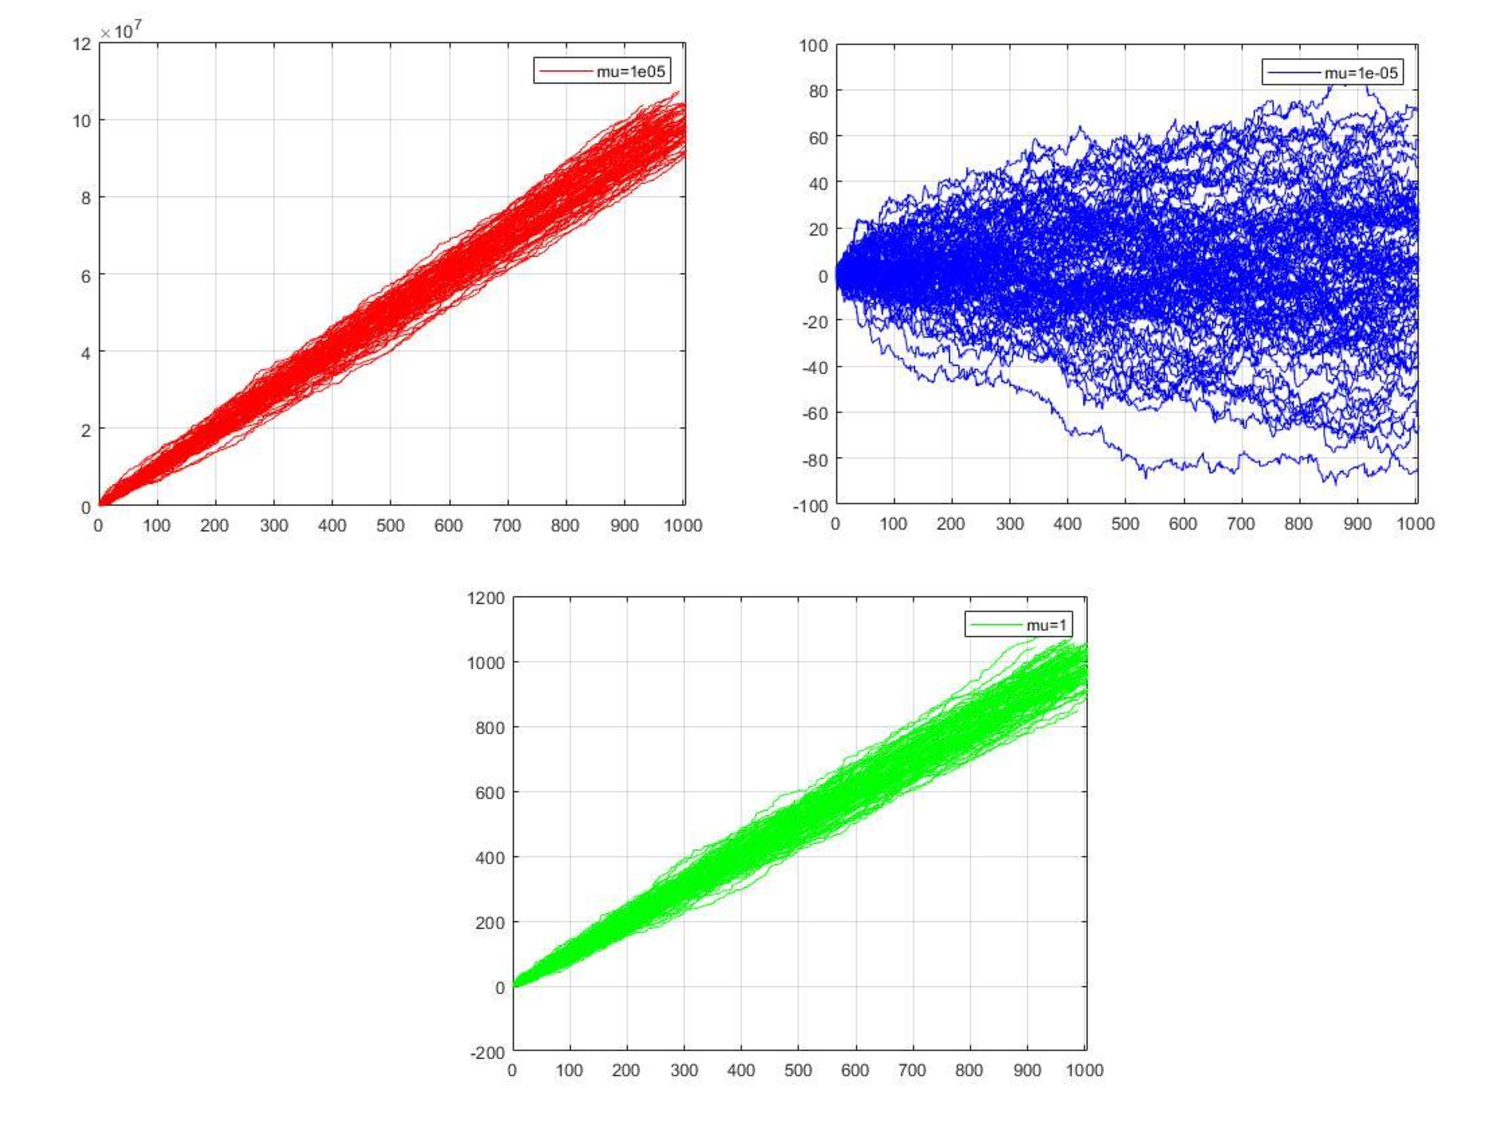
\includegraphics[scale=0.65]{figures/Task3/Diff_mu.pdf}
    \caption{Path with different $\mu$}
    \label{fig:diffmu}
\end{figure}

\subsection{Different $\sigma$}
Similarly, to verify $\sigma$, both $\mu$ and $\lambda$ are set to $1$.

$\sigma$ determines the variance for $X_t$. When $\sigma=10^{5}$, as shown on Figure \ref{fig:diffsigma}, the variance become very large as $\sigma$ is large. Consider a 100 loops simulation the variance among $A_{1000}$ is $9.982\times 10^{12}$ which is quite close to theoretical value ($1.0\times 10^{13}$)

If $\sigma$ becomes extreme small, $10^{-5}$, the motion again control by the linear drift and the variance of end values is $1.109\times 10^{3}$ and the theoretical result is $1.0\times 10^{3}$. 
\begin{figure}[H]
    \centering
    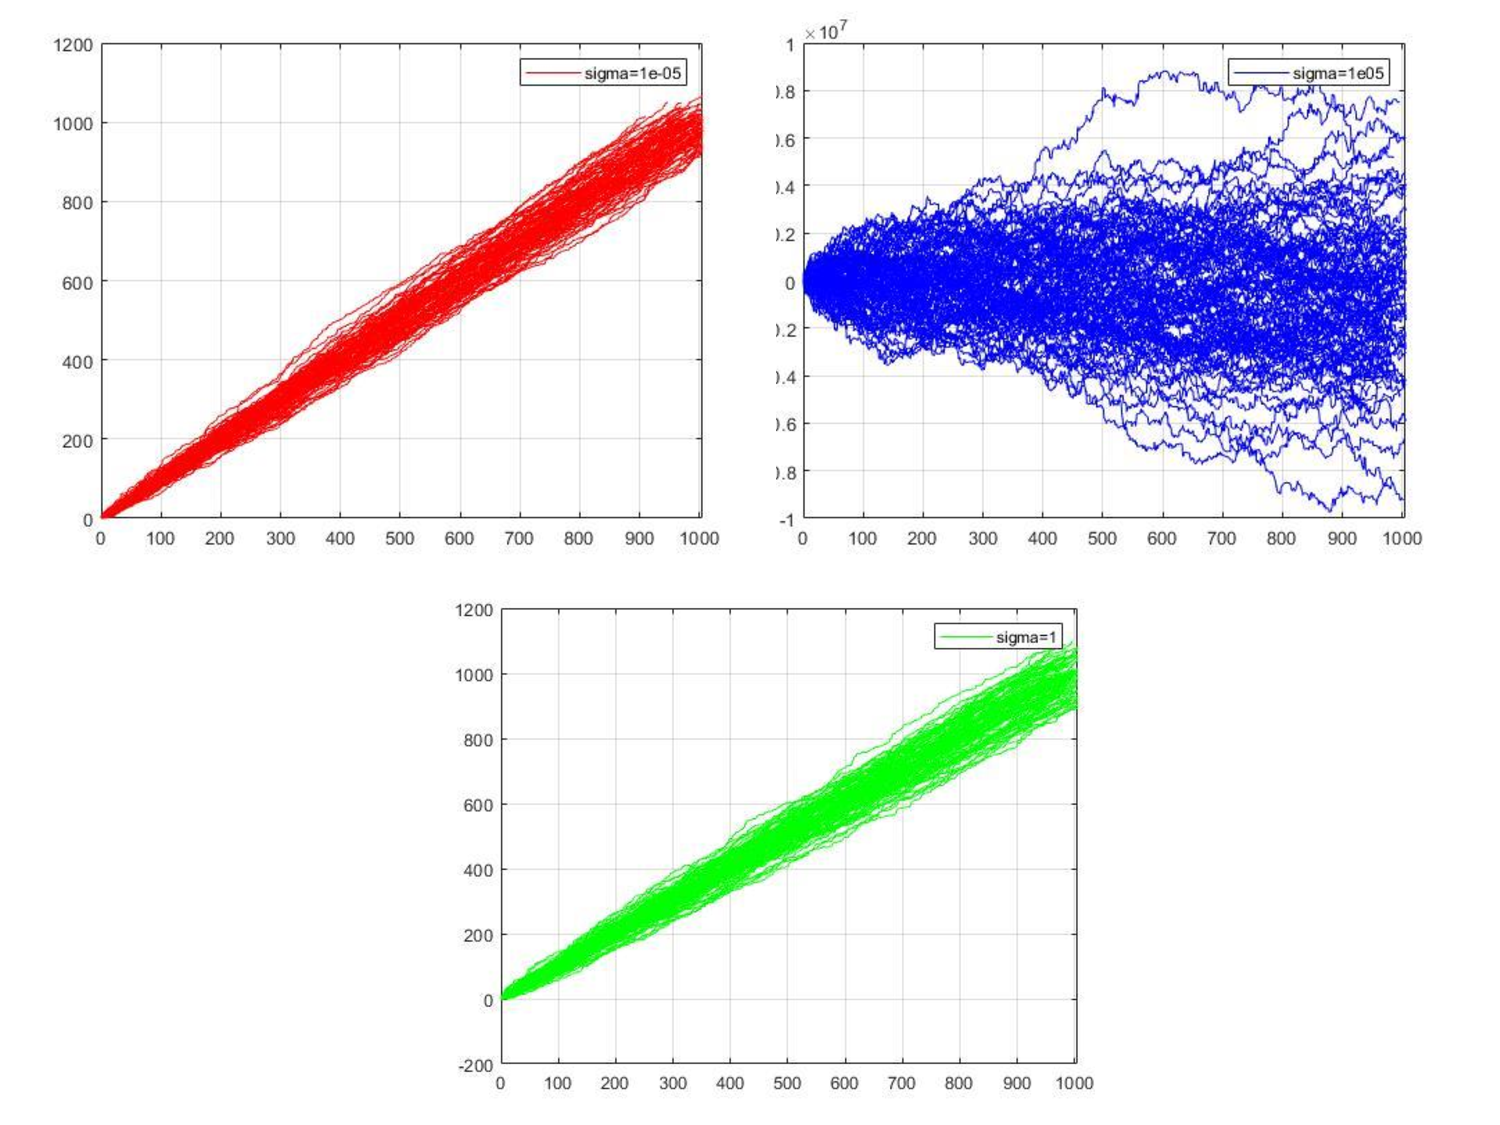
\includegraphics[scale=0.65]{figures/Task3/Diff_sigma.pdf}
    \caption{Path with different $\sigma$}
    \label{fig:diffsigma}
\end{figure}

\subsection{Different $\lambda$}
The $\lambda$ determines the time interval of $T$ and the total time $S$ that is Erlang distribution. If $\lambda$ is very large ($10^{5}$), both $T$ and $S$ are very small that indicates movement are basic only from origin to y-axle, as Figure \ref{fig:difflambda} shows. But when the $\lambda$ is set to $10^{-5}$, $T$ and $S$ are quite large which specifies it takes much more time to finish the entire path motion.
\begin{figure}[H]
    \centering
    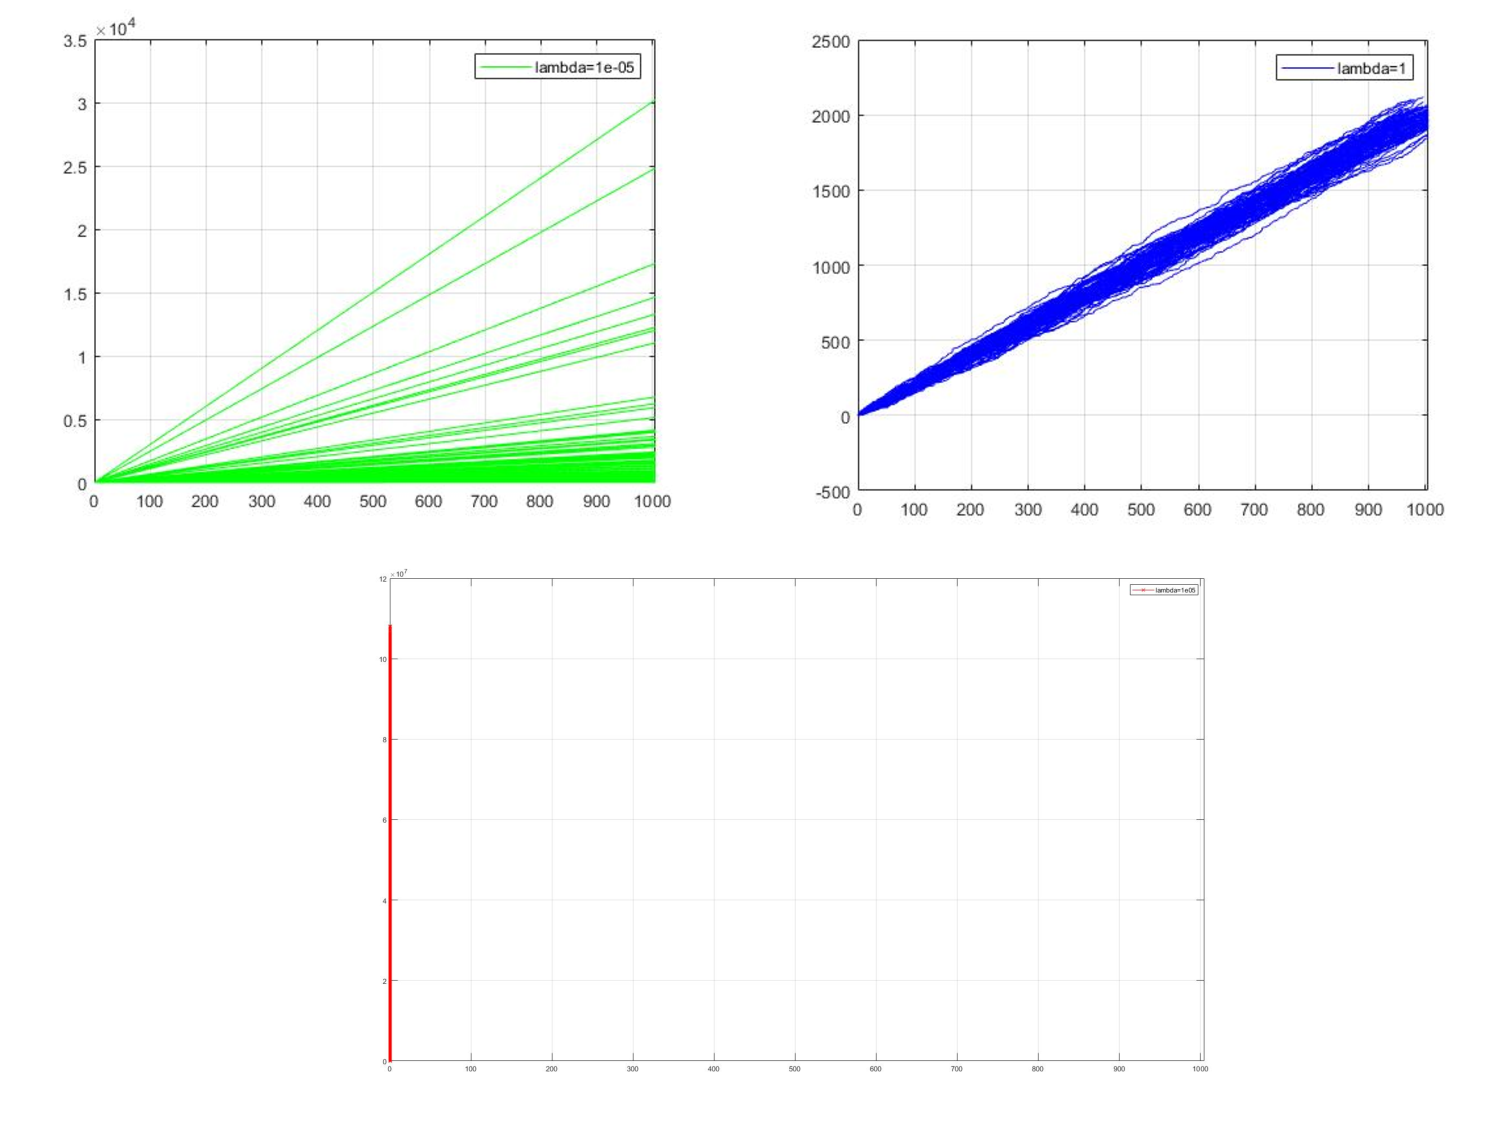
\includegraphics[scale=0.65]{figures/Task3/Diff_lambda.pdf}
    \caption{Path motion with different $\lambda$  }
    \label{fig:difflambda}
\end{figure}

\subsection{$\mu$ vs. $\lambda_Y$} \label{4.4}
Take the jump into consideration, in the situation of $\mu=-1$ and $\lambda_Y=1$, it indicates the linear drift can be counteracted by the jump, then the path becomes like the case of $\mu$ is pretty small, the Brownian motion without linear drift. 
\begin{figure}[H]
    \centering
    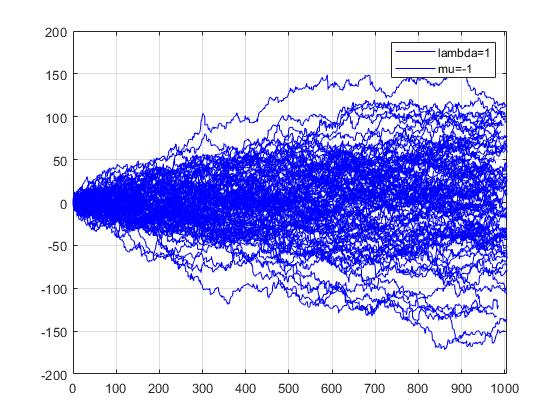
\includegraphics[scale=0.6]{figures/Task3/lambda=1mu=-1.jpg}
    \caption{Simulation result with $\mu=-1$ and $\lambda_Y=1$}
    \label{fig:my_label}
\end{figure}

%\subsubsection{$\mu$ vs. $\sigma$}
%In the case of 









\newpage